% --------------------------------------------	
% Autogenerated LaTeX file for articles 			
% --------------------------------------------	
\ifx\pdfoutput\undefined
\documentclass[,a4paper,10pt,twoside,twocolumn,]{article}
\else
\documentclass[pdftex,,a4paper,10pt,twoside,twocolumn,]{article}
\fi
\label{id206771}\usepackage{ifthen}
% --------------------------------------------
% Check for PDFLaTeX/LaTeX 
% --------------------------------------------
\newif\ifpdf
\ifx\pdfoutput\undefined
\pdffalse % we are not running PDFLaTeX
\else
\pdfoutput=1 % we are running PDFLaTeX
\pdftrue
\fi
% --------------------------------------------
% Load graphicx package with pdf if needed 
% --------------------------------------------
\ifpdf
\usepackage[pdftex]{graphicx}
\pdfcompresslevel=9
\else
\usepackage{graphicx}
\fi

		\usepackage{anysize}
		\marginsize{2cm}{2cm}{2cm}{2cm}
	    \renewcommand\floatpagefraction{.9}
	    \renewcommand\topfraction{.9}
	    \renewcommand\bottomfraction{.9}
	    \renewcommand\textfraction{.1}
	\usepackage{fancyhdr}
\pagestyle{plain}\renewcommand{\headrulewidth}{0.4pt}
\renewcommand{\footrulewidth}{0.4pt}
% ---------------------- 
% Most Common Packages   
% ---------------------- 
\usepackage{makeidx} 
%\usepackage{cite}         
%\renewcommand\citeleft{(}  % parentheses around list
%\renewcommand\citeright{)} % parentheses around list
\usepackage{latexsym}         
\usepackage{enumerate}         
\usepackage{fancybox}      
\usepackage{float}       
\usepackage{ragged2e}       
\usepackage{fancyvrb}         
\makeatletter\@namedef{FV@fontfamily@default}{\def\FV@FontScanPrep{}\def\FV@FontFamily{}}\makeatother
\fvset{obeytabs=true,tabsize=3}
\usepackage{rotating}         
\usepackage{subfigure}         
\usepackage{tabularx}         
\usepackage{url}         
% ---------------
% Document Font  
% ---------------
\usepackage{times}
 \def\keywords{\vspace{-.3em}
 \if@twocolumn
 \small\textit{
Keywords }\/\bfseries---$\!$%
 \else
 \begin{center}\small\bfseries 
Keywords \end{center}\quotation\small
 \fi}
 \def\endkeywords{\vspace{0.6em}\par\if@twocolumn\else\endquotation\fi
 \normalsize\rmfamily}
% --------------------------------------------
% Math support                                
% --------------------------------------------
\usepackage{amsmath,amsthm, amsfonts, amssymb, amsxtra,amsopn}
%\newtheorem{thm}{Theorem}[section]
%\newtheorem{cor}[section]{Corollary}
%\newtheorem{lem}[section]{Lemma}
%\newtheorem{defn}[section]{Definition}
%\newtheorem{prop}[section]{Proposition}
%\newtheorem{ax}{Axiom}
%\newtheorem{theorem}[section]{Theorem}
%\newtheorem{corollary}{Corollary}
%\newtheorem{lemma}{Lemma}
%\newtheorem{proposition}{Proposition}
%\theoremstyle{definition}
%\newtheorem{definition}{Definition}
%\theoremstyle{remark}
%\newtheorem{rem}{Remark}
%\newtheorem*{notation}{Notation}
%\newcommand{\ntt}{\normalfont\ttfamily}
%\newcommand{\thmref}[1]{Theorem~\ref{#1}}
%\newcommand{\secref}[1]{\S\ref{#1}}
%\newcommand{\lemref}[1]{Lemma~\ref{#1}}
 \newcommand{\bysame}{\mbox{\rule{3em}{.4pt}}\,}
 \newcommand{\A}{\mathcal{A}}
 \newcommand{\B}{\mathcal{B}}
 \newcommand{\XcY}{{(X,Y)}}
 \newcommand{\SX}{{S_X}}
 \newcommand{\SY}{{S_Y}}
 \newcommand{\SXY}{{S_{X,Y}}}
 \newcommand{\SXgYy}{{S_{X|Y}(y)}}
 \newcommand{\Cw}[1]{{\hat C_#1(X|Y)}}
 \newcommand{\G}{{G(X|Y)}}
 \newcommand{\PY}{{P_{\mathcal{Y}}}}
 \newcommand{\X}{\mathcal{X}}
 \newcommand{\wt}{\widetilde}
 \newcommand{\wh}{\widehat}
 % --------------------------------------------
 %\DeclareMathOperator{\per}{per}
 \DeclareMathOperator{\cov}{cov}
 \DeclareMathOperator{\non}{non}
 \DeclareMathOperator{\cf}{cf}
 \DeclareMathOperator{\add}{add}
 \DeclareMathOperator{\Cham}{Cham}
 \DeclareMathOperator{\IM}{Im}
 \DeclareMathOperator{\esssup}{ess\,sup}
 \DeclareMathOperator{\meas}{meas}
 \DeclareMathOperator{\seg}{seg}
% --------------------------------------------
% --------------------------------------------
% Load hyperref package with pdf if needed 
% --------------------------------------------
\ifpdf
\usepackage[pdftex,bookmarksnumbered,colorlinks,backref, bookmarks, breaklinks, linktocpage,pdfstartview=FitH]{hyperref}
\else
\usepackage[dvips,bookmarksnumbered,colorlinks,backref, bookmarks, breaklinks, linktocpage,]{hyperref}
\fi
% --------------------------------------------
% ---------------------------------------------- 
% Define a new LaTeX environment (adminipage)    
% ---------------------------------------------- 
\newenvironment{admminipage}%
{ % this code corresponds to the \begin{adminipage} command
 \begin{Sbox}%
 \begin{minipage}%
} %done
{ % this code corresponds to the \end{adminipage} command
 \end{minipage}
 \end{Sbox}
 \fbox{\TheSbox}
} %done
% ---------------------------------------------- 
% Define a new LaTeX length (admlength)          
% ---------------------------------------------- 
\newlength{\admlength}
% ---------------------------------------------- 
% Define a new LaTeX environment (admonition)    
% With 2 parameters:                             
% #1 The file (e.g. note.pdf)                    
% #2 The caption                                 
% ---------------------------------------------- 
\newenvironment{admonition}[2] 
{ % this code corresponds to the \begin{admonition} command
 \hspace{0mm}\newline\hspace*\fill\newline
 \noindent
 \setlength{\fboxsep}{5pt}
 \setlength{\admlength}{\linewidth}
 \addtolength{\admlength}{-10\fboxsep}
 \addtolength{\admlength}{-10\fboxrule}
 \admminipage{\admlength}
 {\bfseries \sc\large{#2}} \newline
 \\[1mm]
 \sffamily
 \includegraphics[width=1cm]{#1}
 \addtolength{\admlength}{-1cm}
 \addtolength{\admlength}{-20pt}
 \begin{minipage}[lt]{\admlength}
 \parskip=0.5\baselineskip \advance\parskip by 0pt plus 2pt
} %done
{ % this code corresponds to the \end{admonition} command
 \vspace{5mm} 
 \end{minipage}
 \endadmminipage
 \vspace{.5em}
 \par
}
% --------------------------------------------
% Commands to manage/style/create floats      
% figures, tables, algorithms, examples, eqn  
% --------------------------------------------
 \floatstyle{ruled}
 \restylefloat{figure}
 \floatstyle{ruled}
 \restylefloat{table}
 \floatstyle{ruled}
 \newfloat{program}{ht}{lop}[section]
 \floatstyle{ruled}
 \newfloat{example}{ht}{loe}[section]
 \floatname{example}{Example}
 \floatstyle{ruled}
 \newfloat{dbequation}{ht}{loe}[section]
 \floatname{dbequation}{Equation}
 \floatstyle{boxed}
 \newfloat{algorithm}{ht}{loa}[section]
 \floatname{algorithm}{Algorithm}
\ifpdf
\DeclareGraphicsExtensions{.pdf,.png,.jpg}
\else
\DeclareGraphicsExtensions{.eps}
\fi
% --------------------------------------------
% $latex.caption.swapskip enabled for $formal.title.placement support
\newlength{\docbooktolatextempskip}
\newcommand{\captionswapskip}{\setlength{\docbooktolatextempskip}{\abovecaptionskip}\setlength{\abovecaptionskip}{\belowcaptionskip}\setlength{\belowcaptionskip}{\docbooktolatextempskip}}
% Guard against a problem with old package versions.
\makeatletter
\AtBeginDocument{
\DeclareRobustCommand\ref{\@refstar}
\DeclareRobustCommand\pageref{\@pagerefstar}
}
\makeatother
% --------------------------------------------
\makeatletter
\newcommand{\dbz}{\penalty \z@}
\newcommand{\docbooktolatexpipe}{\ensuremath{|}\dbz}
\usepackage[latin1]{inputenc}

\def\docbooktolatexgobble{\expandafter\@gobble}
\AtBeginDocument{\ifx\refname\@undefined\let\docbooktolatexbibname\bibname\def\docbooktolatexbibnamex{\bibname}\else\let\docbooktolatexbibname\refname\def\docbooktolatexbibnamex{\refname}\fi}
% Facilitate use of \cite with \label
\newcommand{\docbooktolatexbibaux}[2]{%
  \protected@write\@auxout{}{\string\global\string\@namedef{docbooktolatexcite@#1}{#2}}
}
\newcommand{\docbooktolatexcite}[2]{%
  \@ifundefined{docbooktolatexcite@#1}%
  {\cite{#1}}%
  {\def\@docbooktolatextemp{#2}\ifx\@docbooktolatextemp\@empty%
   \cite{\@nameuse{docbooktolatexcite@#1}}%
   \else\cite[#2]{\@nameuse{docbooktolatexcite@#1}}%
   \fi%
  }%
}
\newcommand{\docbooktolatexbackcite}[1]{%
  \ifx\Hy@backout\@undefined\else%
    \@ifundefined{docbooktolatexcite@#1}{%
      % emit warning?
    }{%
      \ifBR@verbose%
        \PackageInfo{backref}{back cite \string`#1\string' as \string`\@nameuse{docbooktolatexcite@#1}\string'}%
      \fi%
      \Hy@backout{\@nameuse{docbooktolatexcite@#1}}%
    }%
  \fi%
}
% Provide support for bibliography `subsection' environments with titles
\newenvironment{docbooktolatexbibliography}[3]{
   \begingroup
   \let\save@@chapter\chapter
   \let\save@@section\section
   \let\save@@@mkboth\@mkboth
   \let\save@@bibname\bibname
   \let\save@@refname\refname
   \let\@mkboth\@gobbletwo
   \def\@tempa{#3}
   \def\@tempb{}
   \ifx\@tempa\@tempb
      \let\chapter\@gobbletwo
      \let\section\@gobbletwo
      \let\bibname\relax
   \else
      \let\chapter#2
      \let\section#2
      \let\bibname\@tempa
   \fi
   \let\refname\bibname
   \begin{thebibliography}{#1}
}{
   \end{thebibliography}
   \let\chapter\save@@chapter
   \let\section\save@@section
   \let\@mkboth\save@@@mkboth
   \let\bibname\save@@bibname
   \let\refname\save@@refname
   \endgroup
}
% Prevent multiple openings of the same aux file
% (happens when backref is used with multiple bibliography environments)
\ifx\AfterBeginDocument\undefined\let\AfterBeginDocument\AtBeginDocument\fi
\AfterBeginDocument{
   \let\latex@@starttoc\@starttoc
   \def\@starttoc#1{%
      \@ifundefined{docbooktolatex@aux#1}{%
         \global\@namedef{docbooktolatex@aux#1}{}%
         \latex@@starttoc{#1}%
      }{}
   }
}
% --------------------------------------------
% A way to honour <footnoteref>s
% Blame j-devenish (at) users.sourceforge.net
% In any other LaTeX context, this would probably go into a style file.
\newcommand{\docbooktolatexusefootnoteref}[1]{\@ifundefined{@fn@label@#1}%
  {\hbox{\@textsuperscript{\normalfont ?}}%
    \@latex@warning{Footnote label `#1' was not defined}}%
  {\@nameuse{@fn@label@#1}}}
\newcommand{\docbooktolatexmakefootnoteref}[1]{%
  \protected@write\@auxout{}%
    {\global\string\@namedef{@fn@label@#1}{\@makefnmark}}%
  \@namedef{@fn@label@#1}{\hbox{\@textsuperscript{\normalfont ?}}}%
  }
% --------------------------------------------
% Hacks for honouring row/entry/@align
% (\hspace not effective when in paragraph mode)
% Naming convention for these macros is:
% 'docbooktolatex' 'align' {alignment-type} {position-within-entry}
% where r = right, l = left, c = centre
\newcommand{\docbooktolatex@align}[2]{\protect\ifvmode#1\else\ifx\LT@@tabarray\@undefined#2\else#1\fi\fi}
\newcommand{\docbooktolatexalignll}{\docbooktolatex@align{\raggedright}{}}
\newcommand{\docbooktolatexalignlr}{\docbooktolatex@align{}{\hspace*\fill}}
\newcommand{\docbooktolatexaligncl}{\docbooktolatex@align{\centering}{\hfill}}
\newcommand{\docbooktolatexaligncr}{\docbooktolatex@align{}{\hspace*\fill}}
\newcommand{\docbooktolatexalignrl}{\protect\ifvmode\raggedleft\else\hfill\fi}
\newcommand{\docbooktolatexalignrr}{}
\ifx\captionswapskip\@undefined\newcommand{\captionswapskip}{}\fi
% index labelling helper
\def\docbooktolatexprintindex#1{%
   \let\dbtolatex@@indexname\indexname%
   \def\dbtolatex@label{\label{#1}}
   \def\indexname{\dbtolatex@label\let\dbtolatex@label\relax\dbtolatex@@indexname}%
   \printindex
   \let\indexname\dbtolatex@@indexname
   }
\makeatother
\title{\textbf{Article Test Document Title}}
\author{Ramon Casellas}
\begin{document}
{\maketitle\pagestyle{plain}\thispagestyle{empty}}

% --------------------------------------------
% Abstract 
% --------------------------------------------
\begin{abstract}

This article is just a test. This article is just a test. This article is just a test. This article is just a test. This article is just a test. This article is just a test. This article is just a test. This article is just a test. This article is just a test. This article is just a test. This article is just a test. This article is just a test. This article is just a test. This article is just a test. This article is just a test. This article is just a test. This article is just a test. This article is just a test. This article is just a test. This article is just a test. This article is just a test. This article is just a test. This article is just a test. This article is just a test. This article is just a test. This article is just a test. This article is just a test. This article is just a test. This article is just a test. This article is just a test. This article is just a test. This article is just a test. This article is just a test. This article is just a test. This article is just a test. This article is just a test. This article is just a test. This article is just a test. This article is just a test. This article is just a test.
\end{abstract}


This is a {``}short quote{''}.
This is a {``}Quotation with a {`}nested quotation containing a {``}nested quotation and another {`}nested quotation{'}{''}{'}{''}.

\begin{Verbatim}[,fontfamily=default]
This is a literal layout
  It'll be a <pre> until the chunk.pl
script    fixes   things    up.
\end{Verbatim}

This article is just a test. This article is just a test. This article is just a test. This article is just a test. This article is just a test. This article is just a test. This article is just a test. This article is just a test. This article is just a test. This article is just a test.

% figure ------------------------------------------------------
\begin{figure}[hbt]
\begin{center}%
\hypertarget{testfig}{}%

\begin{Verbatim}[]
This is a
  ProgramListing
\end{Verbatim}
\caption{{{Test Figure}}}
\label{testfig}
\end{center}
\end{figure}


This para contains an xref to a figure: \hyperlink{testfig}{Figure {\ref{testfig}}}.

% figure ------------------------------------------------------
\begin{figure}[hbt]
\begin{center}%
\hypertarget{testfig2}{}%

\begin{Verbatim}[]
A Second
  Test Figure
\end{Verbatim}
\caption{{{Test Figure2}}}
\label{testfig2}
\end{center}
\end{figure}


This para contains an \hyperlink{testfig2}{link} to a figure.

\begin{itemize}
%--- Item
\item 
\url{http://www.somewhere.com/asp?php_jsp-\string&fcksup}


%--- Item
\item 
\href{http://wwww.aaaaaaaa.bbbbbb.c.d.fr/aaa/bbb/ccc/ddd/eee/fff/ggg}{AAABBBCCCDDD}
        \url{http://wwww.aaaaaaaa.bbbbbb.c.d.fr/aaa/bbb/ccc/ddd/eee/fff/ggg}

\end{itemize}

\begin{itemize}
%--- Item
\item 
Test item.


%--- Item
\item 
Test item.


%--- Item
\item 
Test item.

\end{itemize}

\begin{enumerate}
%--- Item
\item 
Test item.


%--- Item
\item 
Test item.


%--- Item
\item 
Test item.

\end{enumerate}

This article is just a test. This article is just a test. This article is just a test. This article is just a test. This article is just a test. This article is just a test. This article is just a test. This article is just a test. This article is just a test. This article is just a test. This article is just a test. This article is just a test. This article is just a test. This article is just a test. This article is just a test. This article is just a test. This article is just a test. This article is just a test. This article is just a test. This article is just a test. This article is just a test. This article is just a test. This article is just a test. This article is just a test. This article is just a test. This article is just a test. This article is just a test. This article is just a test. This article is just a test. This article is just a test. This article is just a test. This article is just a test. This article is just a test. This article is just a test. This article is just a test. This article is just a test. This article is just a test. This article is just a test. This article is just a test. This article is just a test.

% figure ------------------------------------------------------
\begin{figure}[hbt]
\begin{center}%
\hypertarget{fig}{}%

{{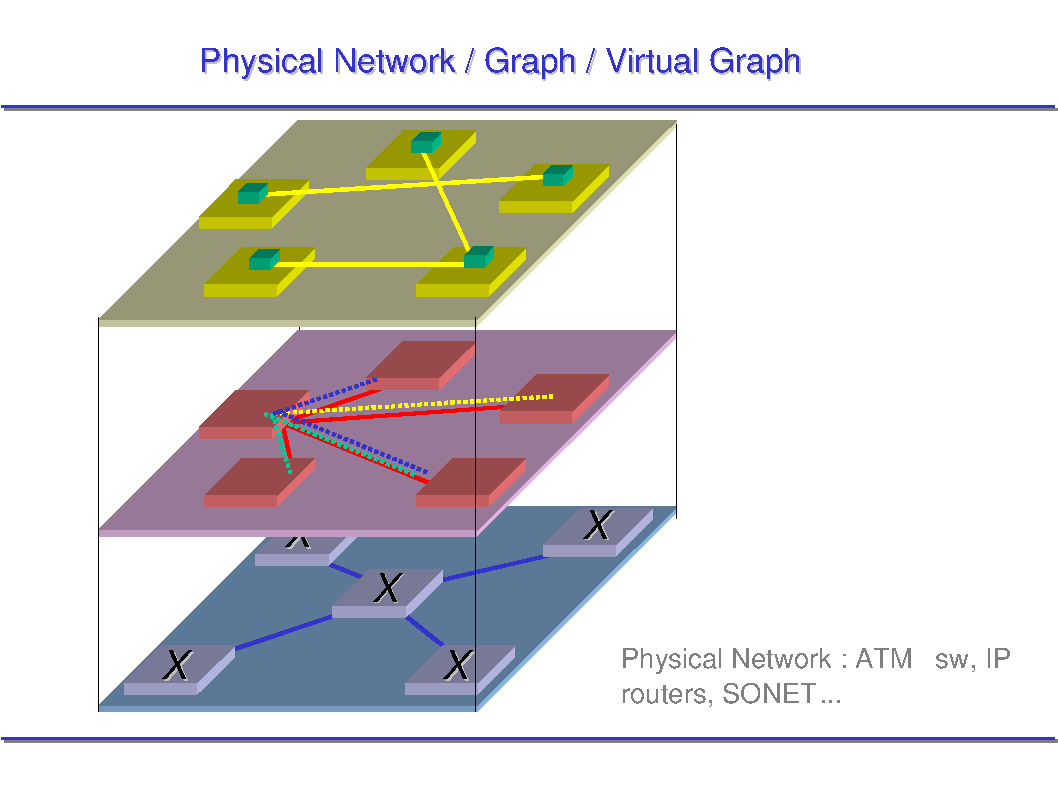
\includegraphics[width=7cm]{figures/sample}}}
\caption{{{A pdf/eps fig}}}
\label{fig}
\end{center}
\end{figure}


% ------------------------   
% Section 
\section{Lists, of course}
\label{id185646}\hypertarget{id185646}{}%

\begin{tabular*}{\linewidth}{ll} 
IBM's Java performance research  & \href{http://www.somewhere.com/asp?php_jsp-\&fcksup?}{http://www.somewhere.com/asp?php\_jsp-\&fcksup}  \\
C vs. Java speed comparisons  & \url{http://www.aceshardware.com/Spades/read.php?article_id=153}  \\
Java versus C++  & \url{http://www.multimania.com/lefevre/java/ceaxx.html}  \\
Java Performance  & \url{http://hepunx.rl.ac.uk/hep2java/meeting/16-03-2000/hoschek2/sld001.htm}  \\
Java Grande Forum  & \url{http://www.javagrande.org/}  \\
Java for Scientific Computing  & \url{http://www.npac.syr.edu/projects/javaforcse/}  \\
The Java HotSpot Performance Engine Architecture  & \url{ http://java.sun.com/products/hotspot/whitepaper.html}  \\
\end{tabular*}

\textbf{No operator overloading} 
For non-primitive types, operator can't be overloaded. There are attractions in allowing operator overloading to support mathematical operations where the notation is close to the normal mathematical formalism and one can take advantage of the operator precedence rules.



\textbf{No automatic type narrowing.} 
The type conversion which could lead to a loss of precision doesn't happen automatically, but variables must be cast explicitly. This protects the developer from certain hard-to-find bugs and makes the behaviour of the code explicit, but some may find it annoying.




% ------------------------   
% Section 
\section{First level section}
\label{id186254}\hypertarget{id186254}{}%

\subsection{Second level section}
\label{id186260}\hypertarget{id186260}{}%

\subsubsection{Section}
\label{id186267}\hypertarget{id186267}{}%

\newcommand{\dbappendix}[1]{\section{#1}}%
% ------------------------------------------------------------- 
% Appendixes start here
% -------------------------------------------------------------
\appendix

% -------------------------------------------------------------
% appendix:  Appendix 
% ------------------------------------------------------------- 	
\dbappendix{Appendix}
\label{id186280}\hypertarget{id186280}{}%

This is just a test.

This article is just a test. This article is just a test. This article is just a test. This article is just a test. This article is just a test. This article is just a test. This article is just a test. This article is just a test. This article is just a test. This article is just a test.

This article is just a test. This article is just a test. This article is just a test. This article is just a test. This article is just a test. This article is just a test. This article is just a test. This article is just a test. This article is just a test. This article is just a test.

This article is just a test. This article is just a test. This article is just a test. This article is just a test. This article is just a test. This article is just a test. This article is just a test. This article is just a test. This article is just a test. This article is just a test.

This article is just a test. This article is just a test. This article is just a test. This article is just a test. This article is just a test. This article is just a test. This article is just a test. This article is just a test. This article is just a test. This article is just a test.

This article is just a test. This article is just a test. This article is just a test. This article is just a test. This article is just a test. This article is just a test. This article is just a test. This article is just a test. This article is just a test. This article is just a test.

This article is just a test. This article is just a test. This article is just a test. This article is just a test. This article is just a test. This article is just a test. This article is just a test. This article is just a test. This article is just a test. This article is just a test.
% ------------------------------------------- 
%
%  Bibliography
%
% ------------------------------------------- 
\let\oldbibname\bibname
\let\oldrefname\refname
\def\bibname{A Test Bibliography}
\let\refname\bibname
\section*{\docbooktolatexbibnamex}\hypertarget{bib1}{}

\begin{docbooktolatexbibliography}{WIDELABEL}{\subsection}{Books}\hypertarget{id186326}{}

% -------------- biblioentry 
\bibitem[ASU96]{ASU96}\docbooktolatexbibaux{id186332}{ASU96}
\hypertarget{id186332}{\emph{Compilers, Principles, Techniques, and Tools}}, Alfred V. Aho, Ravi Sethi, and Jeffrey D. Ullman, Addison-Wesley Publishing Company, Copyright \copyright{} 1996 Bell Telephone Laboratories, Inc., 0-201-10088-6, James T. DeWolf.


\end{docbooktolatexbibliography}

\begin{docbooktolatexbibliography}{WIDELABEL}{\subsection}{Periodicals}\hypertarget{id186440}{}

% -------------- biblioentry 
\bibitem[Abbrev]{Abbrev}\docbooktolatexbibaux{id186576}{Abbrev}
\hypertarget{id186576}{\emph{A Really Full BiblioEntry}}, AuthorFirstname AuthorSurname, Copyright \copyright{} 1998 Copyright holder, EditorFirstName EditorSurname, ISBN, PageNums, PubDate, PubPublisherNameAny StreetAnywhere, XX99999USA, ReleaseInfo.


% -------------- biblioentry 
\bibitem[Walsh97]{Walsh97}\docbooktolatexbibaux{walsh97}{Walsh97}
\hypertarget{walsh97}{\emph{}}, .


\end{docbooktolatexbibliography}
\let\bibname\oldbibname
\let\refname\oldrefname

% --------------------------------------------
% End of document
% --------------------------------------------
\end{document}
